\section{Résultats supplémentaires}
\label{sec:supp}

\begin{figure}[h]
    \centering
    \begin{subfigure}{0.5\textwidth}
        \centering
        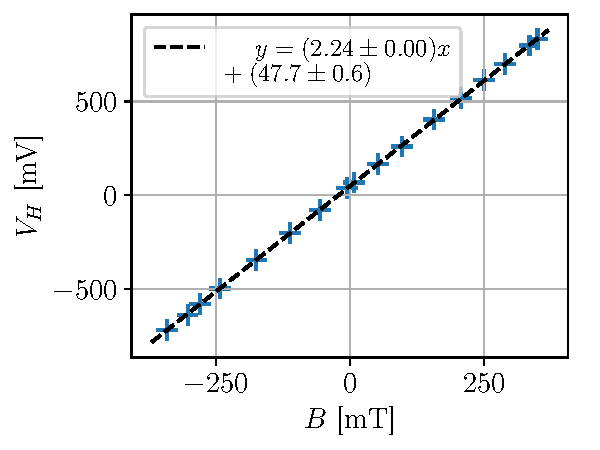
\includegraphics[width=\textwidth]{figures/U(B),InP1micro.pdf}
        \caption{}
    \end{subfigure}%
    \begin{subfigure}{0.5\textwidth}
        \centering
        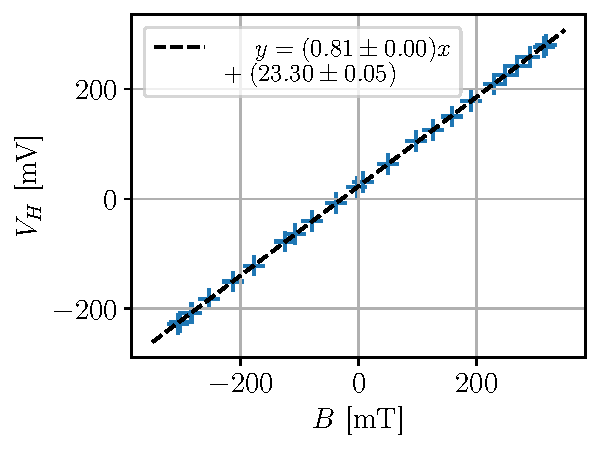
\includegraphics[width=\textwidth]{figures/U(B),InP2micro.pdf}
        \caption{}
    \end{subfigure}
    \caption{Tension en fonction de la norme signée du champ magnétique pour l'échantillon InP d'épaisseur (a) 1 \si{\micro\meter} (b) 2 \si{\micro\meter}}
    \label{fig:inpV(B)}
\end{figure}

\begin{figure}[h]
    \centering
    \begin{subfigure}{0.5\textwidth}
        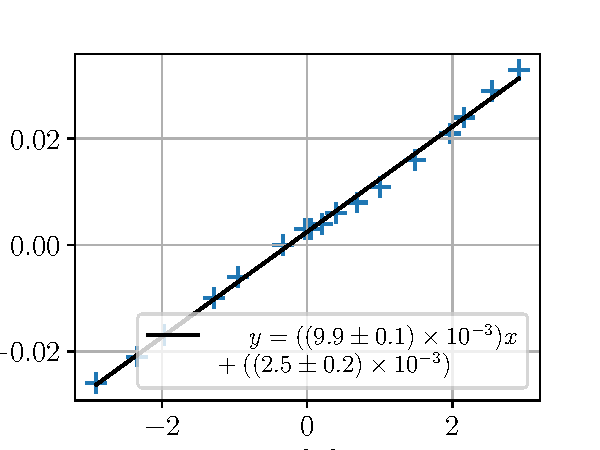
\includegraphics[width=\linewidth]{figures/Ag_I.pdf}
        \caption{}
        \label{fig:Ag_I}
    \end{subfigure}%
    \begin{subfigure}{0.5\textwidth}
        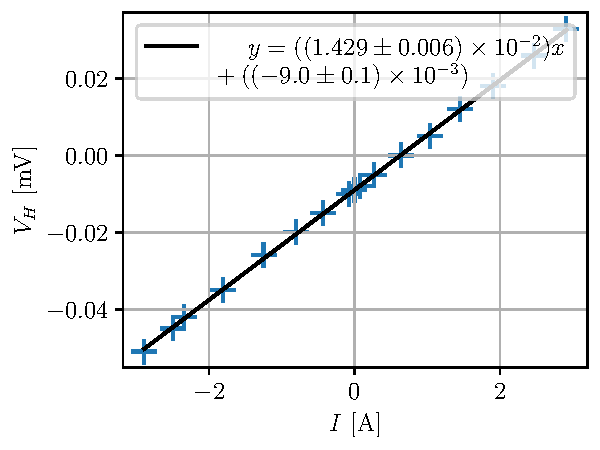
\includegraphics[width=\linewidth]{figures/Cu_I.pdf}
        \caption{}
        \label{fig:Cu_I}
    \end{subfigure}
    \begin{subfigure}{0.5\textwidth}
        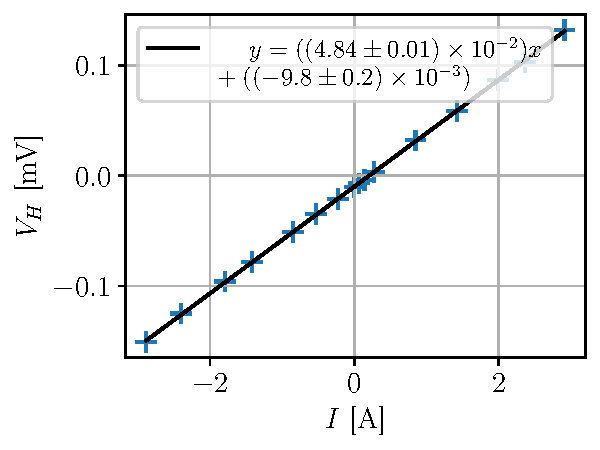
\includegraphics[width=\linewidth]{figures/Bi_I.pdf}
        \caption{}
        \label{fig:Bi_I}
    \end{subfigure}
    \caption{Régression de \(V_H\) en fonction de \(I\) à \(B\) constant pour (a) Ag, (b) Cu et (c) Bi}
    \label{fig:5branch_I}
    \vspace*{1cm}
\end{figure}


\begin{table}[h]
    \centering
    \begin{tabulary}{\textwidth}{C C C C}
        \toprule
        échantillon & \(\alpha_I = \frac{V_H}{I}\) & \(R_H = -\frac{\alpha_I a}{B}\) & N [\si{\per \cubic \meter}] \\
        \midrule
        Ag & \((9.9 \pm 0.1) \times 10^{-3}\) & \((-5.5 \pm 0.2) \times 10^{-11}\) & \((1.14 \pm 0.04) \times 10^{29}\) \\
        Cu & \((1.429 \pm 0.006) \times 10^{-2}\) & \((-6.5 \pm 0.2) \times 10^{-11}\) & \((9.6 \pm 0.2) \times 10^{28}\) \\
        Bi & \((4.84 \pm 0.01) \times 10^{-2}\) & \((-3.94 \pm 0.09) \times 10^{-7}\) & \((1.59 \pm 0.03) \times 10^{25}\) \\
        \bottomrule
    \end{tabulary}
    \caption{Valeurs de \(R_H\) et \(N\) obtenues pour les échantillons à 5 branchements à \(B\) constant}
    \label{tab:5branch_I}
\end{table}


\section{Calcul d'erreurs}
\label{sec:erreurs}

Les erreurs sur les mesures sont données dans le \autoref{tab:erreurs}.

\begin{table}[h]
    \centering
    \begin{tabulary}{\textwidth}{C C C}
        \toprule
        Variable & Erreur & Commentaire \\
        \midrule
        \(a\) [\si{\micro\meter}] & 0.01 & Estimation grossière basée sur l'epaisseur indiquée sur les échantillons \\
        \(B\) [\si{\milli\tesla}] & \(1\% + 3\textrm{ lsd}\) & Indiqué sur le manuel du teslamètre \\
        \(V\) [\si{\milli\volt}] & \(0.01\) & Estimation basée sur la variation des valeurs affichées \\
        \(I\) [\si{\milli\ampere}] & \(0.001\) & Estimation basée sur la variation des valeurs affichées \\
        \(I\) [\si{\ampere}] & \(0.01\) & Estimation basée sur la variation des valeurs affichées \\
        \bottomrule
    \end{tabulary}
    \caption{Erreurs estimées sur les mesures}
    \label{tab:erreurs}
\end{table}

\paragraph*{Regression linéaire}
Les erreurs sur les fits linéaires \(y = ax + b\) sur les mesures \((x_i, y_i) ; i = \{1, \hdots, n\}\) sont donnés par l'\autoref{eq:erreur:fit} \cite{erreursmesure}:

\begin{equation}
    \label{eq:erreur:fit}
    \begin{aligned}
        (\Delta a)^2 &= \frac{\sum_{i=1}^{n}(y_i - (a x_i + b))^2}{(n-2) \sum_{i=1}^{n}(x_i - \bar{x})^2}\\
        \Delta b &= \bar{x} \Delta a + a \Delta \bar{x}
    \end{aligned}
\end{equation}

En pratique, ces valeurs sont calculées par la bilbiothèque python \texttt{numpy}.

\paragraph*{Equations}
Les erreurs sur \(R_H\) et \(N\)sont données par les équations suivantes:

\begin{equation}
    \label{eq:erreur:Rh_B}
    \Delta R_H = |\frac{a}{I}|\Delta \alpha_B + |\frac{a \alpha_B}{I^2}|\Delta I + |\frac{\alpha_B}{I}|\Delta a
\end{equation}

\begin{equation}
    \label{eq:erreur:Rh_I}
    \Delta R_H = |\frac{a}{B}|\Delta \alpha_I + |\frac{a \alpha_I}{B^2}|\Delta B + |\frac{\alpha_I}{B}|\Delta a
\end{equation}

\begin{equation}
    \label{eq:erreur:N}
    \Delta N = |\frac{1}{q R_H^2}|\Delta R_H
\end{equation}

En supposant qu'il n'y a aucune erreur sur q la charge élémentaire d'un électron qui est une valeur tabulée.
Toutes ces erreurs sont calculées en pratique par la bibliothèque \texttt{uncertainties}.
